        \documentclass{standalone}
        \usepackage{../BlogTikz}
        \begin{document}

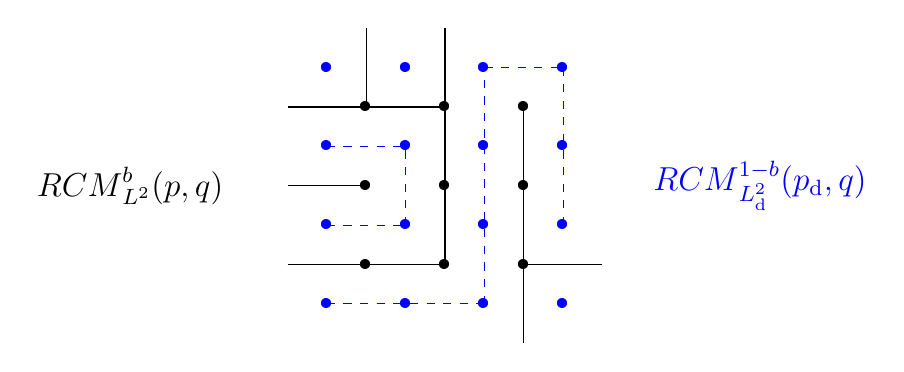
\begin{tikzpicture}[scale=1]
\tikzstyle{every node}=[font=\small]
	\draw (-2,1) to (0,1);
	\draw (-2,0) to (-1,0);
	\draw (-2,-1) to (0,-1); \draw (1,-1) to (2,-1);
	\draw (-1,1) to (-1,2);
	\draw (0,-1) to (0,2);
	\draw (1,-2) to (1,0); \draw (1,1) to (1,0);

	\foreach \XCoord in {-1,0,1}{
		\foreach \YCoord in {-1,0,1}{
			\node at (\XCoord, \YCoord) {\textbullet};
		}
	}

	\draw[blue, dashed] (0.5,1.5) to (1.5,1.5);
	\draw[blue, dashed] (-1.5,0.5) to (-0.5,0.5);
	\draw[blue, dashed] (-1.5,-0.5) to (-0.5,-0.5);
	\draw[blue, dashed] (-1.5,-1.5) to (0.5,-1.5);
	\draw[blue, dashed] (-0.5,-0.5) to (-0.5,0.5);
	\draw[blue, dashed] (0.5,-1.5) to (0.5,1.5);
	\draw[blue, dashed] (1.5,-0.5) to (1.5,1.5);

	\foreach \XCoord in {-1.5,-0.5,0.5,1.5}{
		\foreach \YCoord in {-1.5,-0.5,0.5,1.5}{
			\node at (\XCoord, \YCoord) {\textcolor{blue}{\textbullet}};
		}
	}

	\node at (-4,0) {\large$\operatorname{RCM}_{\mathbb{L}^2}^b(p,q)$};
	\node at (4,0) {\large\textcolor{blue}{$\operatorname{RCM}_{\mathbb{L}_{\mathrm{d}}^2}^{1-b}(p_\mathrm{d},q)$}};
\end{tikzpicture}
        \end{document}
